\section{Our Method}

\subsection{Overview}

{\color{red} Using DETR model as our example to verify the acceleration of transformer, }

The overall DETR architecture is surprisingly simple and described in Figure xxx. It contains three main components, which we represent below:
a CNN backbone to extract a compact feature map, an encoder-decoder transformer model, and a simple feed neural network (FFN) which is composed
of two-layers of $1 \times 1$ convolutions with ReLU activation functions. In this work, we take DETR as our example to accelerate the inference
time on NVIDIA GeForce RTX 2080Ti GPU and our main efforts are put on the transformer part. \\

DPOF is an automated operators fusion strategy module. The whole architecture of automatically generating tensor program is shown in Figure xxx.
The input of DPOF is a configuration of un-optimized deep neural network with any operator fusion. Each operator in the computation graph is 
tagged with a type label to determine whether it is fused with other adjacent operators or not. After running through the DPOF module, each operator is given a new tag, and adjacent operators are merged into subgraphs according to the relationship of the predicted tags. The system
then generates the high-performance tensor programs on GPUs for these subgraphs. Therefore, our system has four major components: 
(1) a DPOF module that finds an optimized operator fusion schedule for the transformer model.
(2) a subgraph scheduler module that allocates time resources for optimizing multiple subgraphs genereated by the DPOF module.
(3) a program sampler module that delineates a large search space and randomly samples various programs from it.
(4) a performance tuner module that trains a cost model to measure the performance of sampled tensor programs.


\begin{figure*}[htbp]
    \centering
    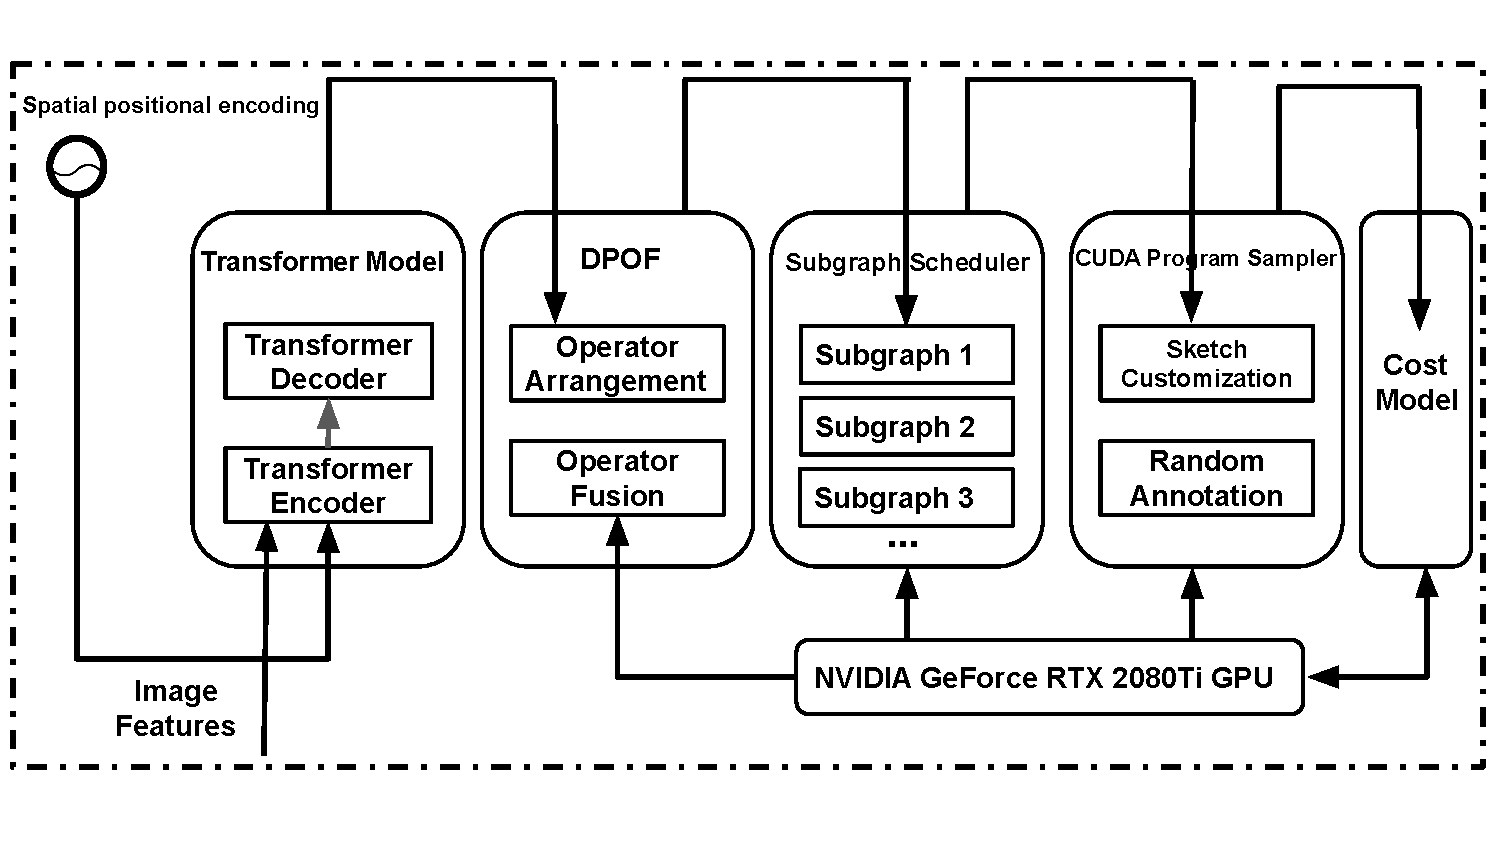
\includegraphics[height=7cm, width=18cm]{figs/fig3}
    \caption{xxx}
    \label{fig:fig3}
\end{figure*}


\subsection{DPOF}


\subsubsection{Operator Arrangement}
% computation graph -> computation queue and move all of the placeholder operators -> set all of the operators in queue as opaque type and get the 
% maximum phases of our scheduling.
To find an optimized schedule for a transformer model, we first use topological sort algorithm to obtain the execution order of the computation operators in the 
original graph. Second, we build a computation queue to store these operators. It is convenient for us to find a good scheduling based on the queue rather than 
computation graph.For the placeholder variables, we do not consider them because they only stores the input and output of the computation results and does 
not mitigate the performance of the whole graph. As mentioned in the operator pattern section, each operator has its own type and the different types of the same 
operator make the difference in the runtime. Third, we set all of the operators as opaque type and assume that there is no fusion relationship with each other.
The size of such queue is the maximum number phase of the scheduling algorithm which is defined in problem definition.


\subsubsection{Operator Fusion}
When we get the execution order of the computation operators and the maximum number phase of our schedule, we partition the original computation graph
$G=(V, E)$ into $V-V^{'}$ and $V^{'}$. The edges in set of $V-V^{'}$ have the pointing relationship with the edges in set of $V{'}$. That is, all of the 
edges start from $V-V^{'}$ and end up with $V{'}$. We call $V{'}$ the segmentation set.

\begin{figure}[htbp]
    \centering
    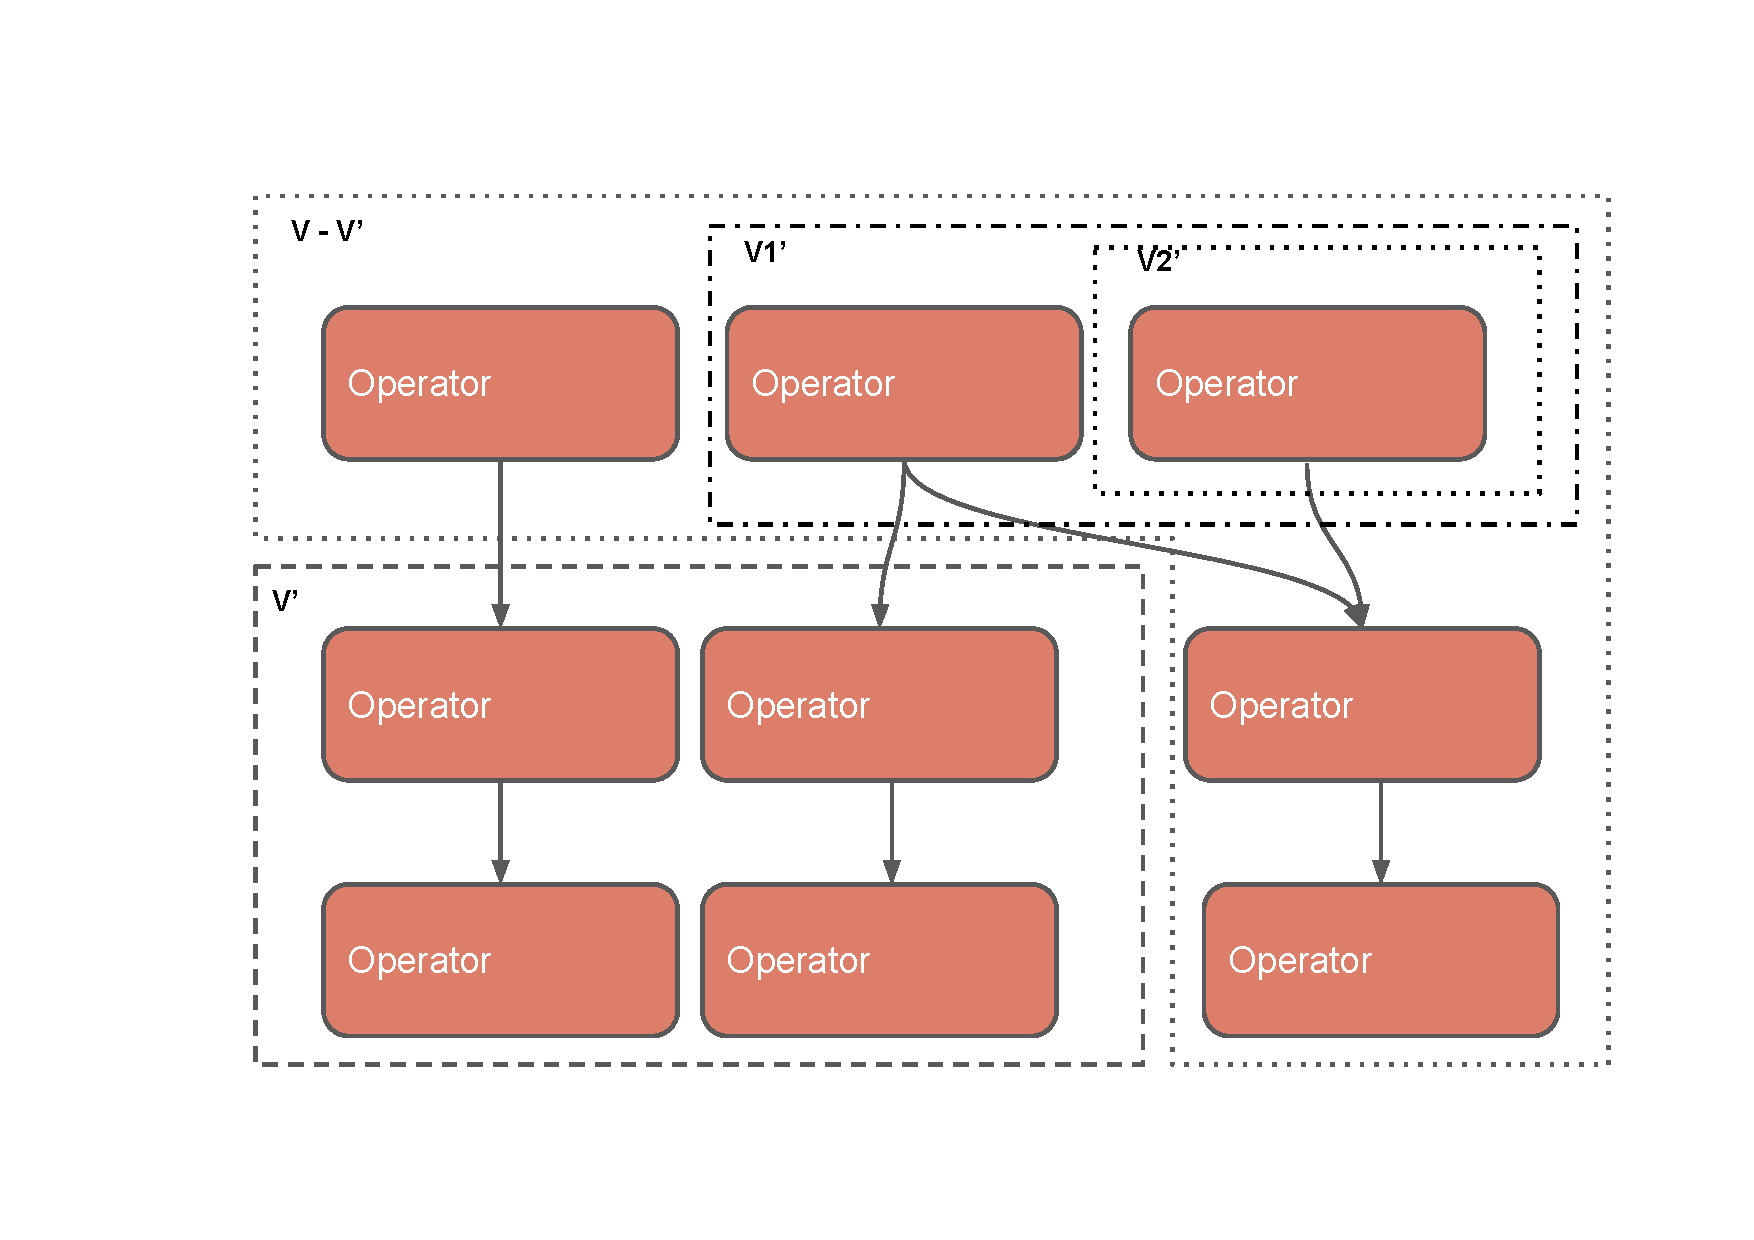
\includegraphics[height=6cm, width=6cm]{figs/fig2}
    \caption{xxx}
    \label{fig:fig1}
\end{figure}

The relationship is illustrated in Figure xxx. We can find that there are lots of segmentaion sets in the computation graph. Following the dynamic programming
pipeline, we can enumerate the segmentaion sets $V{'}$ of $V$ and convert the problem to a sub-problem that attains the optimial schedule for $V-V^{'}$. Therefore,
the whole graph can be sovled by employing the segmentaion set recursively. \\
We define $dp[V]$ as the latency of the graph with the node set $V$ under an optimial schedule $S$. And then we define $temp[V^{'}]$ as the latency of 
phase $(V^{'}, F)$. In the representation, $F$ is the better fusion strategy for the segmentaion set $V^{'}$. Consequently, we can get the state transition 
equation as follows,
\begin{equation}
    dp[V] = min_{ v \in V^{'}}(dp[V-V^{'}] + \sum_{v}temp[v]),    
\end{equation}
where $v$ is the node in segmentaion set $V^{'}$ and the boundary value of the state transition equation is $dp[\varnothing] = 0$. In order to get the optimial
schedule, we store the each node $v$ in segmentaion set $V^{'}$ that can make the latency of each $V$ in $action[V]$.
Following the above information, we implement the operator fusion scheduling as shown in Algorithm xxx.

% \begin{algorithm}[htb]
%     \caption{Operator Fusion Strategy}
%     \label{fra:Framwork}
%     \begin{algorithmic}[1]
%       \Require
%         % The set of positive samples for current batch, $P_n$;
%         % The set of unlabelled samples for current batch, $U_n$;
%         % Ensemble of classifiers on former batches, $E_{n-1}$;
%         a computation graph $G=(V, E)$ with the opaque type for ${\forall v \in V}, pattern(v) = 0$;
%       \Ensure
%         % Ensemble of classifiers on the current batch, $E_n$;
%         A operator fusion strategy with the type of each operator $v \in V, pattern(v)$;

%     \State \textbf{function} func1(G)
%       \State Extracting the set of reliable negative and/or positive samples $T_n$ from $U_n$ with help of $P_n$;
%       \label{code:fram:extract}
%       \State Training ensemble of classifiers $E$ on $T_n \cup P_n$, with help of data in former batches;
%       \label{code:fram:trainbase}
%       \State $E_n=E_{n-1}cup E$;
%       \label{code:fram:add}
%       \State Classifying samples in $U_n-T_n$ by $E_n$;
%       \label{code:fram:classify}
%       \State Deleting some weak classifiers in $E_n$ so as to keep the capacity of $E_n$;
%       \label{code:fram:select} \\
%       \Return $E_n$;
%     \end{algorithmic}
% \end{algorithm}


\begin{algorithm}[htb]
    \setstretch{0.8}
    \caption{Operator Fusion Strategy}
    \begin{algorithmic}[1]
        \Require
        % The set of positive samples for current batch, $P_n$;
        % The set of unlabelled samples for current batch, $U_n$;
        % Ensemble of classifiers on former batches, $E_{n-1}$;
        a computation graph $G=(V, E)$ with the opaque type for ${\forall v \in V}, pattern(v) = 0$;
      \Ensure
        % Ensemble of classifiers on the current batch, $E_n$;
        A operator fusion strategy with the type of each operator $v \in V, pattern(v)$;
        \\
        \State Defining $dp[\varnothing] \gets 0$, $dp[V] \gets +\infty$, $action[V] \gets \varnothing$;
        \State Defining $S \gets \left[\varnothing\right]$ (a stack to store the phase of optimial schedule for operator fusion);
    \\
    \Function {SelectSchedule}{$G$}
        \State $V$ = all operators in computation graph $G$;
        \State Scheduler(V);
        % \State $S = \left[ \qquad \right]$
        \While{$V \neq \varnothing $}
            \State $V^{'}, F = action[V]$;
            \State Put phase $(V^{'}, F)$ into the stack $S$;
            \State $V = V - V^{'}$
        \EndWhile
        \State \Return {the Fusion Strategy $S$}

    \EndFunction
    \\
    \Function{Scheduler}{V}
        \If{$dp[V] \neq +\infty$} 
            \State \Return{dp[V]}
        \EndIf
        \ForAll{$v \in V^{'}$}
            \State $T_{V^{'}}, F_{V^{'}} = PhasePartition(V^{'})$
            \State $T_{V} = Scheduler(V-V^{'}) + \sum_{v_i \in V^{'}}T_{V^{'}}$
            \If{$T_{V} \le dp[V]$}
                \State $dp[V] = T_{V}$
                \State $action[V] = (V^{'}, F_{V^{'}})$
            \EndIf
        \EndFor;
        \State \Return{$dp[V]$}
    \EndFunction
    \\
    \Function{PhasePartition}{$V^{'}$}
        % \If{ $type(v_i \in V^{'} ) == compute\_matmul$}
        %     \State Partition $V^{'}$ into separate groups based cut point $v_i$;
        % \Else
        %     \State xxx
        % \EndIf

        \ForAll{$operators \ v_i \in \ V^{'}$} 
            \If{$pattern(v_i, v_j)\neq opaque$} 
                \State $T_{fused(i, j)} = Runtime(pair(v_i, v_j))$
            \Else
                \State $T_{fused(i, j)} = +\infty$
            \EndIf
        \EndFor
        % \State \Return{$T_{fused(i, j)}, "fused v_i and v_j into an operator"$}        
        \State \Return{$T_{fused(i, j)}, pattern(v_i, v_j)$}        

    \EndFunction




    %     \If {$left < right$}
    %         \State $middle \gets (left + right) / 2$
    %         \State $result \gets result +$ \Call{MergerSort}{$Array, left, middle$}
    %         \State $result \gets result +$ \Call{MergerSort}{$Array, middle, right$}
    %         \State $result \gets result +$ \Call{Merger}{$Array,left,middle,right$}
    %     \EndIf
    %     \State \Return{$result$}
    % % \EndFunction

    %   \ForAll {$c$ such that $c\in RecentMBatch(E_{n-1})$}
    %     \label{code:TrainBase:getc}
    %     \State $T=T\cup PosSample(c)$;
    %     \label{code:TrainBase:pos}
    %   \EndFor;
    %   \For{$i=1$; $i<n$; $i++$ }
    %     \State $//$ Your source here;
    %   \EndFor
    %   \For{$i=1$ to $n$}
    %     \State $//$ Your source here;
    %   \EndFor
    %   \State $//$ Reusing recent base classifiers.
    %   \label{code:recentStart}
    %   \While {$(|E_n| \leq L_1 )and( D \neq \phi)$}
    %     \State Selecting the most recent classifier $c_i$ from $D$;
    %     \State $D=D-c_i$;
    %     \State $E_n=E_n+c_i$;
    %   \EndWhile
      \label{code:recentEnd}
    \end{algorithmic}
  \end{algorithm}


\subsection{Subgraph Scheduler}

% Using topological sort to build a queue, then extract feature from each operator to generate schedule. 
% When tunning a transformer model, our goal is to reduce the model's latency, meeting latency requirements, or
% minimizing tuning time when tuning no longer improves the performance of subgraph significantly.

{\color{red} Change the cost model of the task scheduler, make it early stopping for large kernel}
A transformer model can be partitioned into kinds of independent subgraphs (such as batch\_matmul + softmax). In the process of 
optimization, spending time to tune some subgraphs does not improve the whole performance of entire computation graph. As mentioned in the Ansor paper, there
are two reasons: (1) the subgraph is not a performance bottleneck, or (2) tuning brings only minimal improvement in the subgraph\'s performance. Therefore, we
should dynamically allocate different amounts of time resources to different kinds of subgraphs. A subgraph can appear multiple times in models because of the 
characteristics of the transformer. We define a task as a process performed to generate high-performance programs for a subgraph. It means that obtaining a high
optimized transformer needs completing lots of tasks. 

When tuning a set of subgraphs in transformer, we combine three types of goals together: (1) reducing the latency of transformer, (2) meeting latency requirements
for a set of subgraphs, or (3) minimizing tuning time when tuning no longer improves the performance of transformer significantly. We define $t$ as the allocation
vector, where $t_i$ is the number of time units spent on \textit{i-}th task and the initial value of $t$ is $(1, 1, ..., 1)$. We also define $g_{i}(t)$ as the minimum subgraph latency under the \textit{i-}th task
with $t_i$ time units. Therefore, the latency of the subgraphs $f(g_{1}(t), g_{2}(t), ..., g_{n}(t))$ can describe the end-to-end latency of a transformer model and our
goal is to minimize this function. In order to minimize the end-to-end latency of the transformer, we define the following objective function:
\begin{equation}
    % dp[V] = min_{ v \in V^{'}}(dp[V-V^{'}] + \sum_{v}temp[v]),   
    % f = \sum\limits_{j=1}^{m} max \left[\sum\limits_{i \in S(j)}w_{i} \times max(g_{i}(t), ES(g_{i}, t)), L_{j} \right] 
    f =  max \left[\sum\limits_{i = 1}^{n} w_{i} \times max(g_{i}(t), ES(g_{i}, t)), L_{j} \right] 
    %{\sum_{i \in S(j) w_{i} \times max(g_{i}(t), ES(g_{i}, t))}}
\end{equation}
In the above function, $w_i$ is the number of appearances of task $i$ in the transformer. We define $L_{j}$ as the latency requirement of subgraph $j$, meaning that we do not want to spend tuning time on a subgraph if its latency 
has already met the requirement. In order to achieve the effect of early stopping, we also define a function named ${ES(g_i, t)}$ by looking at the history of latecny
of \textit{i-}th task. Unlike the objective functions defined in Ansor, we first make a comparison between meeting the requirement and early stopping, and then optimize
each task sequentially. Finally, we use a scheduling algorithm based on gradient descent to efficiently optimize the objective function mentioned in Ansor.


\subsection{Program Sampler}

{\color{red} Add the new derivation rules to generate new sketchs:
cross-thread reduction to optimize batch matmul and softmax}

To sample tensor program effectively that can cover a large search space, we also define a hierarchical search
space with two levels like Anosr: \textbf{sketch} and \textbf{annotation}. We define the high-level structures 
of tensor programs as our sketches and set millions of low-level choices (\textit{e.g.}, blocking size, virtual thread tiling, cooperative fetching) as our annotations. The generated tensor program is composed of two top. The component of the first level are sketches generated
by the derivation rules which are designed on GPU platform. The detail information of the second level are randomly annotated from the annotation
space. In order to generate sketches for a subgraph of transformer (DAG), we visit all the computation nodes in a topological order and iteratively build 
a generation structure. For compute-intensive or the nodes with a high chance of data reuse (such as batch matrix multiplication, convolution2d), we build 
a classic tile and fusion structures for them as the sketch. It is worth noting that some new nodes for caching will also be introduced to increase memory 
usage during the generation of sketch.



Figure \ref{fig:fig4} shows an example of the generated sketches for a common subgraph which contains matrix multiplication and softmax operations. For the example subgraph, 
the sorted order of the five nodes in the DAG is \textbf{(A, B, M, S, D)}. To get the sketches for the subgraph, we start from output node \textbf{D} and apply the rules
defined in Ansor to the computation node one by one. We can get the generated sketch 1 by Anosr in the Figure xxx. From the generated sketch 1, we find that the matrix 
multiplication and softmax operations are performed separately, and they are not integrated into a computation kernel. Fortunately, the derivation-based sketch generation 
in Ansor is flexible enough to generate the required structures for emerging algorithms and hardware, because Ansor allows users to register new derivation rules and integrate
them seamlessly with existing rules. In the next section, I will describe in detail about our sketch customization and fused policy.
% We will explain the sampling process of \textbf{scaled dot-product attention} for GPUs 
\begin{figure*}[htbp]
    \centering
    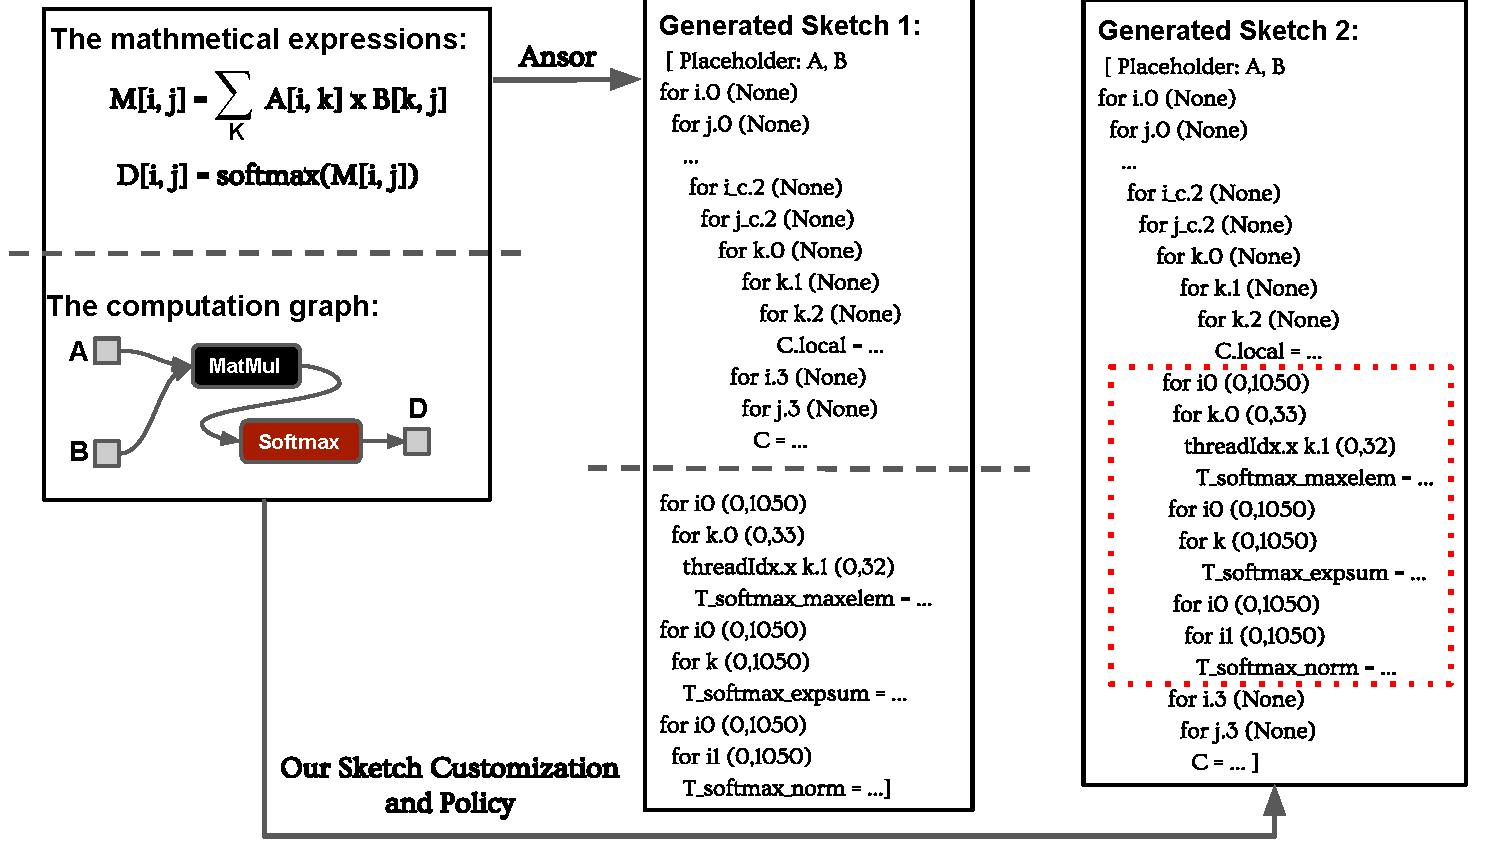
\includegraphics[height=6cm, width=10cm]{figs/fig4}
    % 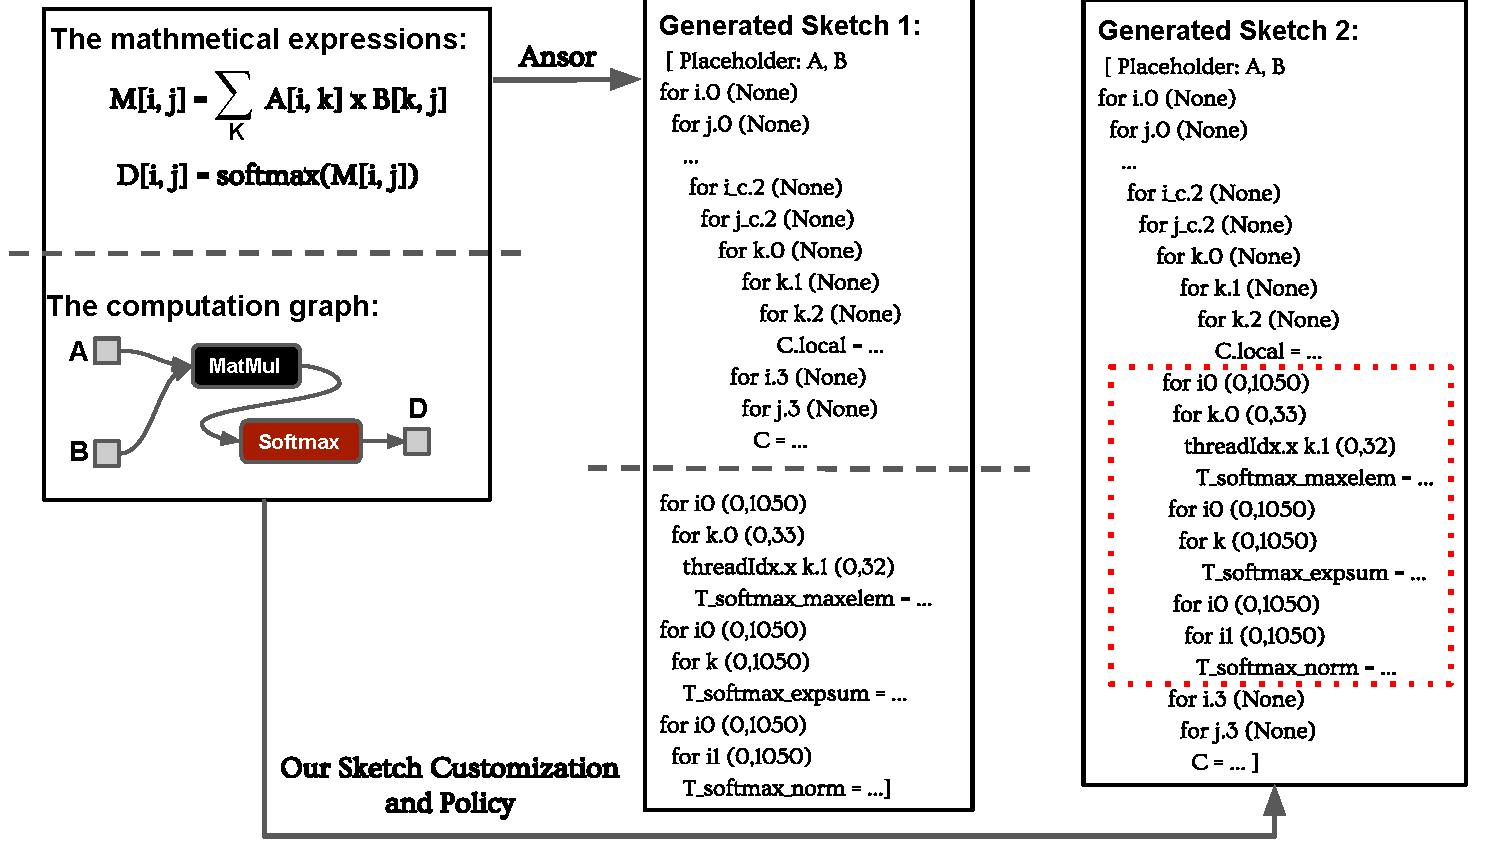
\includegraphics[width=10cm]{figs/fig4}
    % \hspace{1in}
    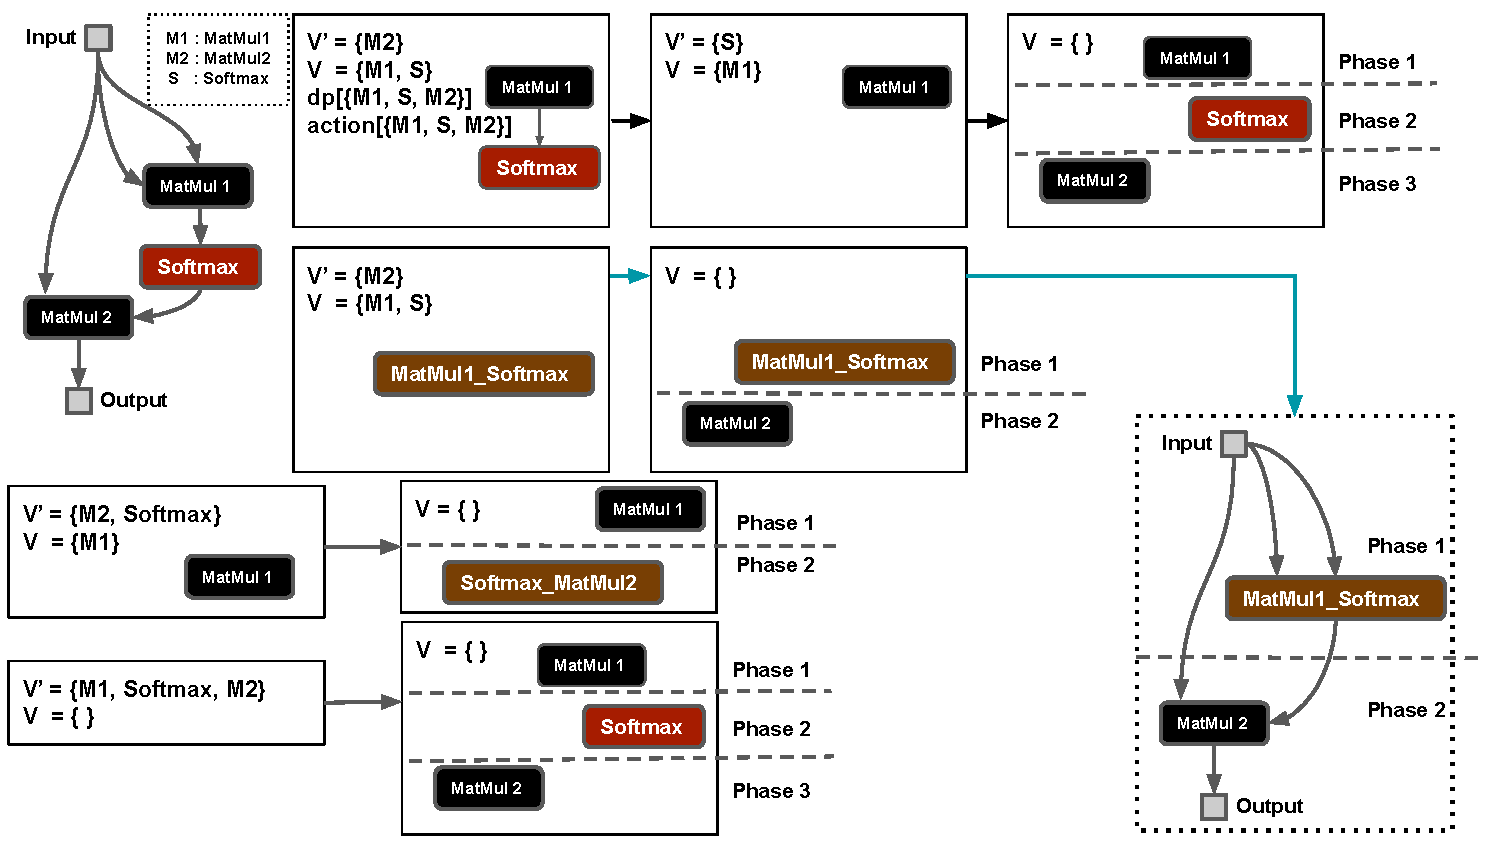
\includegraphics[height=6cm, width=8cm]{figs/fig7}
    \caption{xxx}
    \label{fig:fig4}
\end{figure*}

% \begin{figure}[htbp]
% \centering
% \begin{minipage}[t]{0.48\textwidth}
% \centering
% \includegraphics[width=6cm]{test1.jpg}
% \caption{World Map}
% \end{minipage}
% \begin{minipage}[t]{0.48\textwidth}
% \centering
% \includegraphics[width=6cm]{test2.jpg}
% \caption{Concrete and Constructions}
% \end{minipage}
% \end{figure}



\subsubsection{Sketch Customization} 

The default sketch configuration of Anosr for the multi-level tiling structure to match the GPU backend is SSSRRSRS.
The first three S corresponds to BlockIdx, virtual thread, and ThreadIdx in GPUs programming model, respectively.
The SSSRRSRS tile structure for matrix multiplication expands the original %3-level loop \textbf{(i, j, k)} into a 19-level loop \textbf{(i_{0},j_{0},i_{1},j_{1}, ...)}.
Even if we do not enumerate the loop order, this multi-level tiling structure can take this into consideration. In the example subgraph shown in Figure xxx, we design an effective
operator fusion policy for the sketch generation. The SSSR-RSRS tile structure is for batch matrix multiplication and softmax operators. In order to fuse more opertors and make 
full use of GPUs computation resources, we insert a caching node with the SS-S tile structure to store the sketch generation of the matrix multiplication in it and then 
send it to the sketch generation of softmax to get the final sketch of the subgraph. From the Figure xxx, we can find that the generation sketch of matrix multiplication 
and softmax operators are fused into the same computation kernel.




% \subsubsection{Random Annotation} 
The sketches generated by our customization are incomplete programs because they only have thread parallel structures without specific 
value of these parameters. Therefore, we should turn them into complete programs and then fine-tuning and evaluate the complete programs. 
We randomly pick one sketch from the a list of generated sketches by our customizations. As for the outer loops, we use parallelize intrinstics to optimize them. And for the inner loops, we use vectorize and unroll intrinstics to optimize them.
All valid parameters for the random values are sampled from a uniform distribution.



\subsection{Performance Tuner}

{\color{red} Evolutionary Search and Learned Cost model (same as Ansor)}


\textbf{ML-Based Cost Model and Evolutionary Search:} 
One way to find the best scheduling of the tensor program from a large search space is by auto-tuning. Therefore, a cost model is particularly 
important in the process of evaluating the performance of programs. The extracted features include arithmetic features and memory access features, which
includes number of float operations, number of integer operations, vectorization related features, unrolling related features, parallelization related features,
GPU thread binding related features, buffer access feature, allocation related feature. More specifically, we use weighted squared error as the loss function and 
the loss function of the model $f$ on a sampled program $P$ with throughput $y$ can be defined as follow:
\begin{equation}
    loss(f, P, y) = w_{p}(\sum\limits_{s \in S(P)} f(s) - y)^{2},
\end{equation}
where $S(P)$ is the set of innermost non-loop statements in $P$ and we train a gradient boosting decision tree as the underlying model $f$. In the actual
calculation, we directly make $y$ approximately equal to $w$.\\

A search policy is necessary for the performance tuner. The evolutionary search leverages mutation
and crossover mechanism to generate a new set of candidates repeatedly for several rounds and outputs a small set of programs with the highest scores. The generated
programs will be compiled and measured on the GPU backend to obtain the real running time cost. In the meantime, the collected from the training is then used to
improve the performance of cost model. Therefore, we adopt the search policy which is introduced in Ansor by designing correponding evolution operations to rewrite
and fine-tune the sampled programs.


\label{sec:algo}

